\textcolor{secundario}{\textbf{Valuaci\'on Relativa (\textit{Relative Valuation}).}}\\[5pt]

El perito valuador aplic\'o la metodolog\'ia conocida como Valuaci\'on Relativa (Relative Valuation), mediante el modelo conocido como M\'ultiplos de Cotizaci\'on (Trading Multiples) o \gls{peers}, conforme al enfoque de mercado.\\




%\begin{figure}
%\caption{Modelo de Valuaci\'on Relativa.\label{fig:peers1}}
%
\includegraphics[width=8cm]{\rutaImagenes/peers_1}
%\end{figure}
%
%\begin{figure}
%\caption{PEERS m\'as Utilizados.\label{fig:peers2}}
%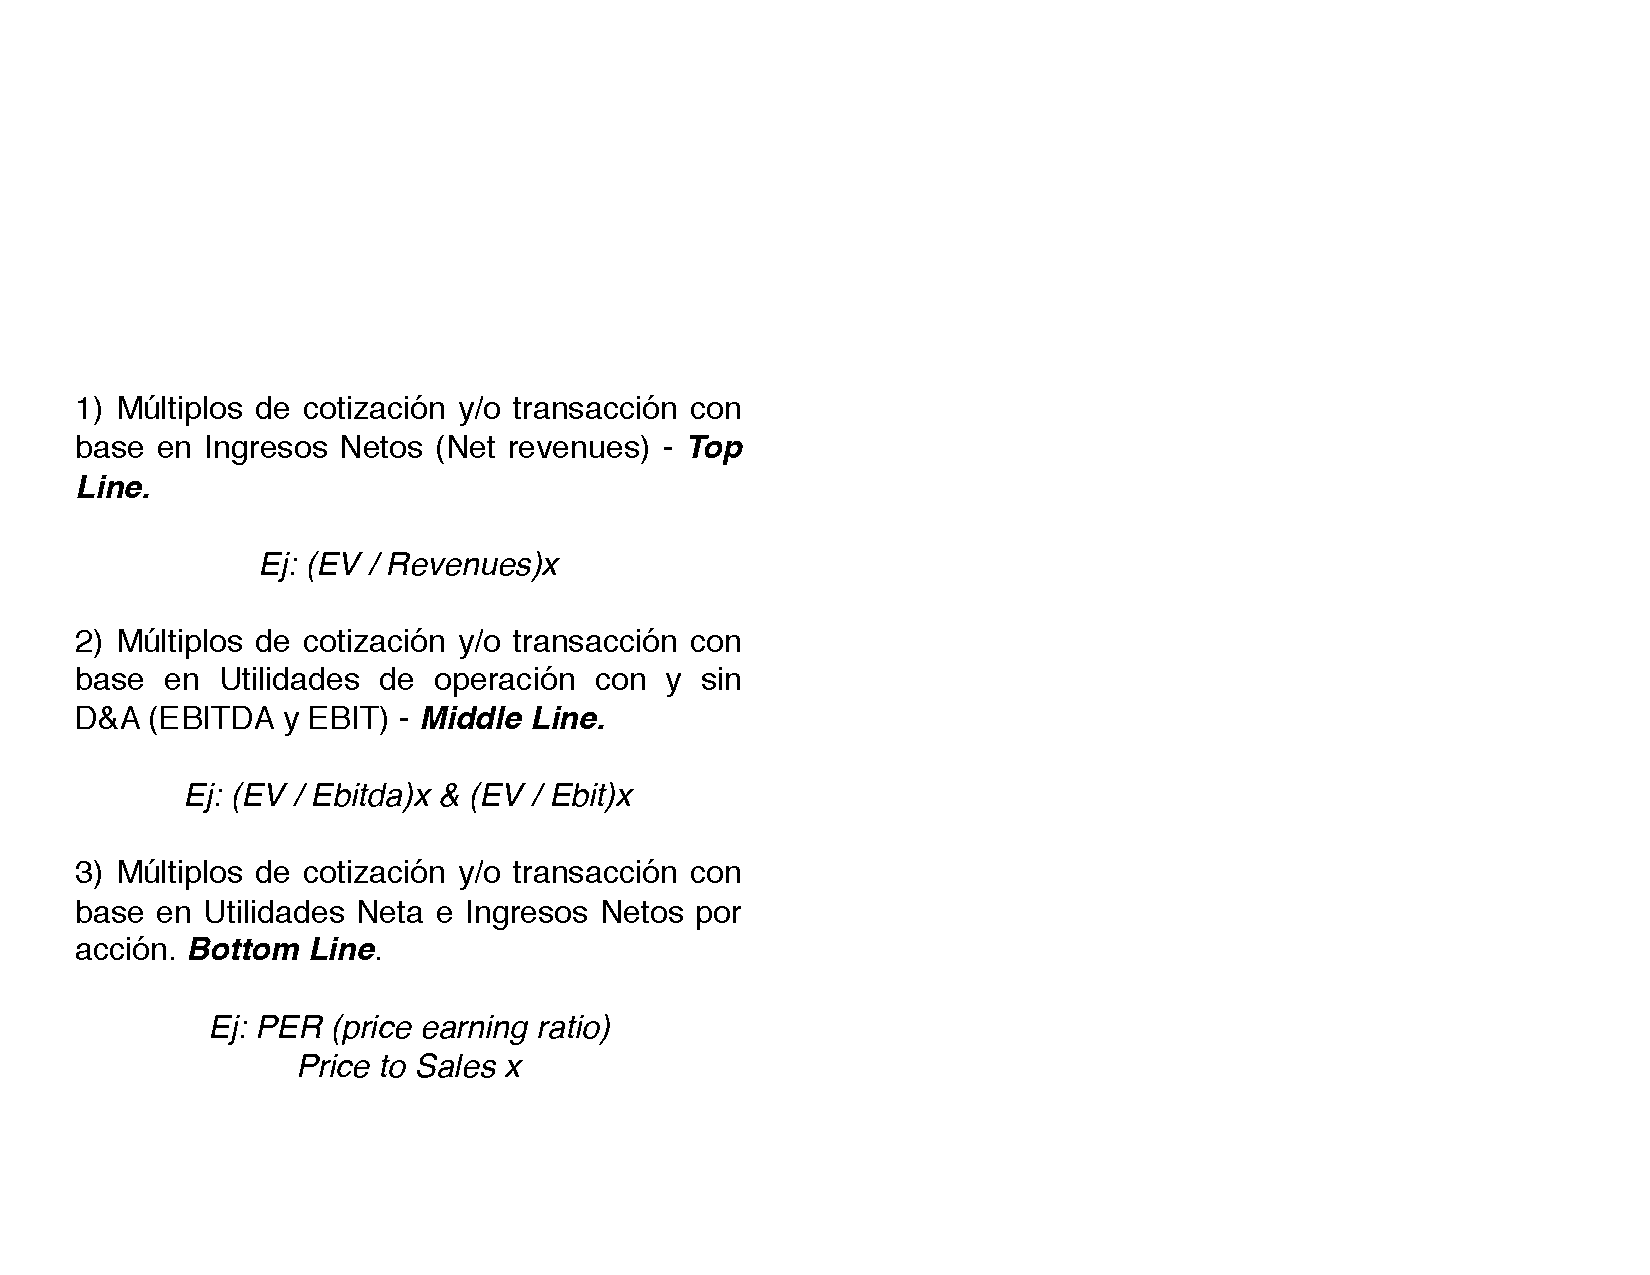
\includegraphics[width=8cm]{\rutaImagenes/peers_2}
%
%\end{figure}
\begin{figure}[H]
\caption{Modelo de Valuaci\'on Relativa. PEERS m\'as utilizados\label{fig:peers1}}
 \raisebox{-0.5\height}{
\includegraphics[width=7cm]{\rutaImagenes/peers_1}}
       \hfill
       \raisebox{-0.5\height}{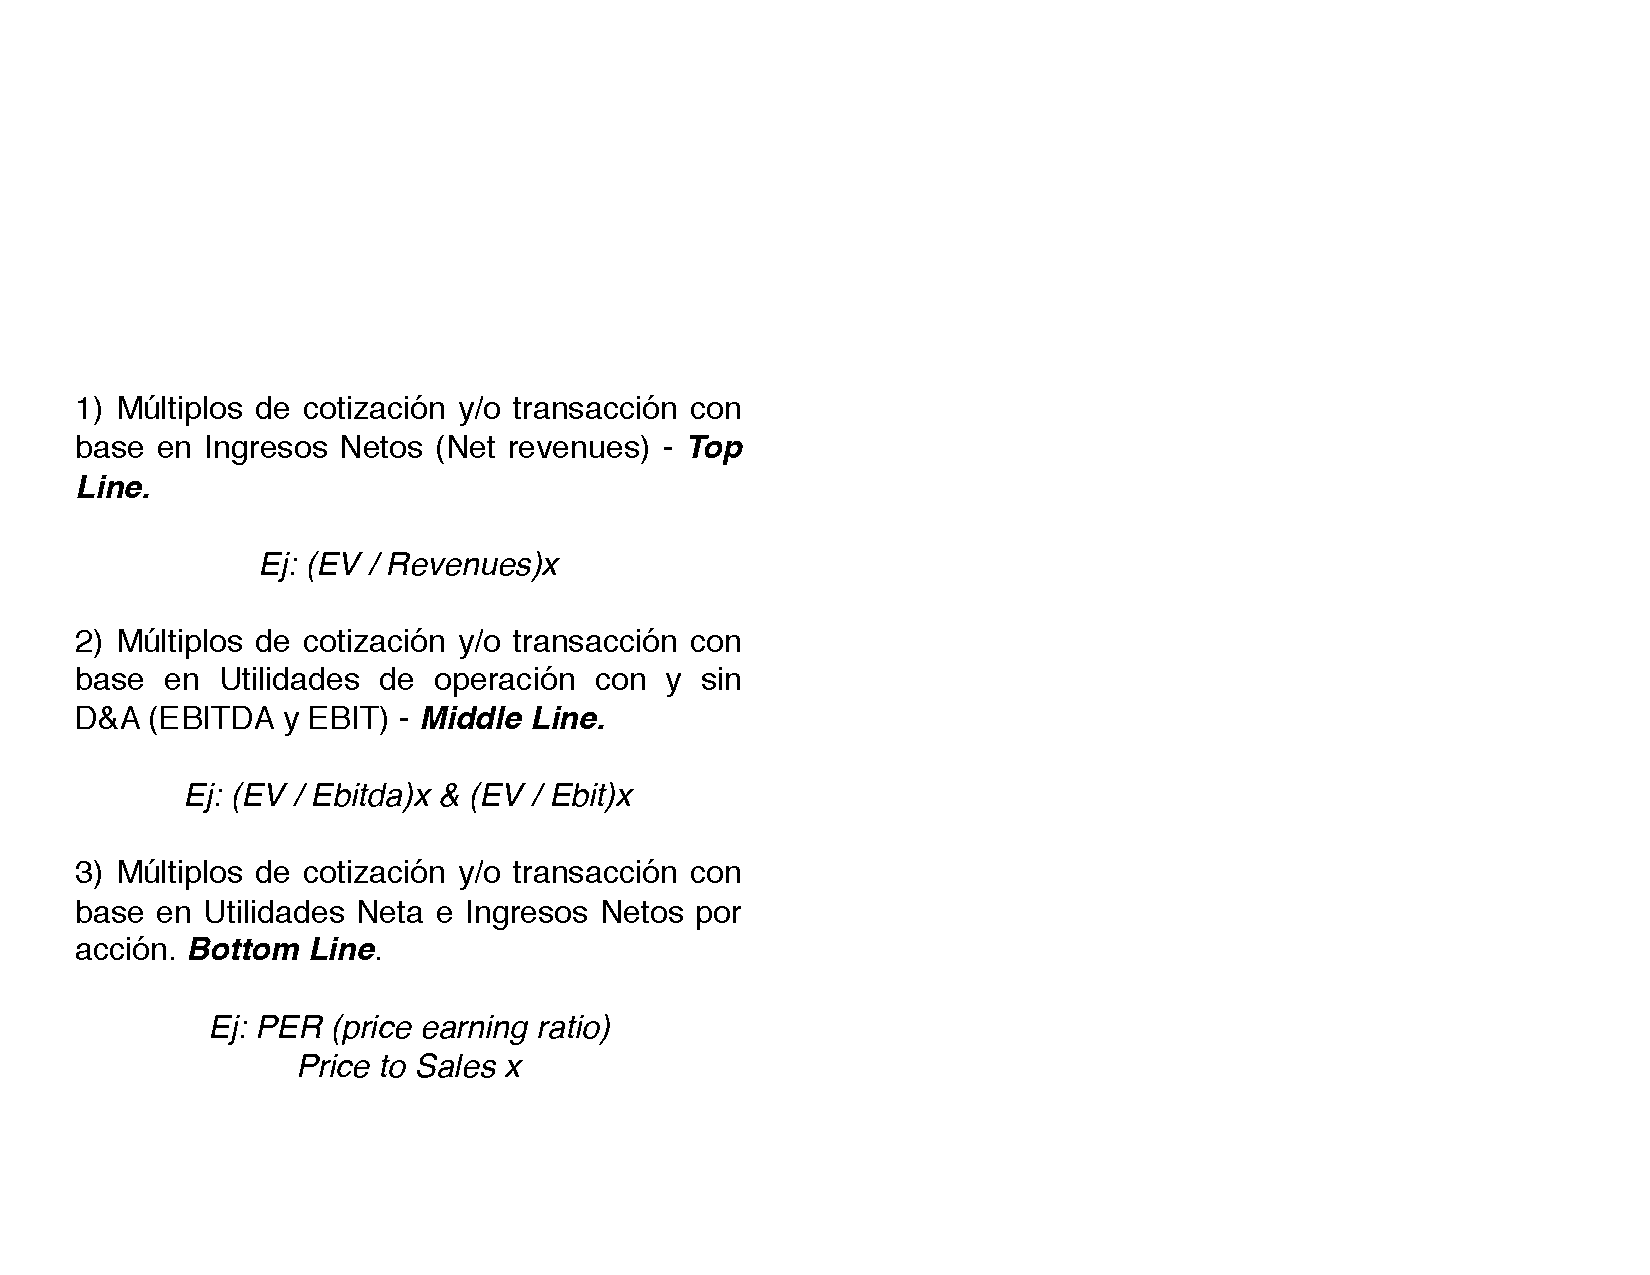
\includegraphics[width=9cm]{\rutaImagenes/peers_2}}
\end{figure}

 Esta metodolog\'ia permite determinar el valor de empresas no cotizadas en bolsa y en el caso de que la empresa objeto de valoraci\'on sea cotizada, el m\'etodo puede ayudarnos a detectar si el mercado  est\'a sobre o infravalorando el valor en cuesti\'on.  A su vez, permite determinar en una valuaci\'on financiera el componente de valor por enfoque de mercado (\textit{\gls{marketaproach}}), utilizando una muestra representativa sobre el m\'ultiplo id\'oneo para el sujeto de valuaci\'on. \\
 